% !TEX root = ../Dissertation.tex
%===================================================================================================

\chapter{Examples}


\section{Section Title}
\label{sec:sectionLabel}

\todo{Write this section.}

\subsection{Subsection Title}
You can \toref{mark things as needing a reference}.

Someone \Citep{Vigouroux1879,Backs1995,BacksS1994} was the first to observe that...
\citep{Backs1995,Firth1973,Vigouroux1879}

See \Cref{fig:edaExample} for a sample figure drawn from a data file.


\fig{You need a figure here}.


%\tikzset{external/remake next} % uncomment this line to force the graphic to be regenerated, even if it's cached from last time.
\begin{figure}
	\centering
	\tikzsetnextfilename{edaExample}
	\begin{tikzpicture}[trim axis left,x=1pt,y=1pt]


	\begin{axis}[width=\textwidth,
			   height=0.5\textwidth,
                           ylabel=Skin Conductance,
                           xlabel=Time (minutes),
                           ytick=\empty,
                           axis x line=bottom, 
                           axis y line=left,
                           enlarge x limits=0.05,
			   enlarge y limits=0.05]
	\addplot[color=red, line width=1,line join=round,cap=round] file {Data/edaExample.csv};
	\end{axis}

	\end{tikzpicture}

	\caption{Typical skin conductance data}
	\label{fig:edaExample}
\end{figure}

\Cref{fig:ecg} is a more elaborate plot.

You can \new{mark something as new to draw Peter's attention to it}

%\fig{Sample ECG}
\begin{figure}[h]
	\centering
	%\includegraphics[width = \textwidth]{Figures/ecg.png}
	%\tikzset{external/remake next}
	\tikzsetnextfilename{ecg}
	\begin{tikzpicture}[trim axis left]
		\begin{axis}[width=0.9\textwidth,
			           height=0.5\textwidth,
		                   xlabel=Time (seconds),
		                   ylabel=Measured voltage,
		                   ytick=\empty,
		                   xtick={0,...,5},
		                   xmax=5,
		                   xmin=0,
		                   axis x line=bottom,
		                   axis y line=left,
		                   enlarge x limits=0.05,
		                   enlarge y limits=0.05,
		                   ]
			\addplot[color=blue,
			             line width=1pt,
			             line join=round,
			             cap=round] file {Data/ecg.csv};

			\coordinate (ArrowStart) at (axis cs:1.2,0.23);
			\coordinate (ArrowEnd) at (axis cs:0.73,0.18);	
			\coordinate (ArrowEndd) at (axis cs:1.4,0.18);	
			
		\end{axis}

		\path[draw=black, line width=1pt,->] 
			(ArrowStart) node[anchor=south] {`R' peaks} -- (ArrowEnd);
		\path[draw=black, line width=1pt,->] 
			(ArrowStart) -- (ArrowEndd); 
			

	
	\end{tikzpicture}

	\caption{A typical electrocardiogram, recorded over about 5 seconds.}
	\label{fig:ecg}
\end{figure}

\Cref{tab:eyeMeasurement} is a good example of a nice table.

\renewcommand{\arraystretch}{4.5}
\begin{table}
	\centering
	\small
	\begin{tabu} to \textwidth {  >{\centering}X[1.5,m] || >{\centering}X[m] >{\centering}X[m] >{\centering}X[m] >{\centering\arraybackslash}X[m] }
	%\hline
	\textbf{Method} & \textbf{Hardware} & \textbf{Intrusiveness} & \textbf{Accuracy} & \textbf{Frame rate} \\
	\hline
	Direct observation & Webcam & Low & $\approx 1$\textdegree & $30$ Hz \\
	Photoelectric viewing & Projected light; photosensors & Low & $3'$ over $30$\textdegree & $1000$ Hz \\
	Reflection & Webcam; light source & Low & $0.5$ -- $1$\textdegree & $30$ Hz \\
	EOG & Multi-channel voltmeter & High & Disputed & $1000$ Hz \\
	Electromagnetic & Metal coils attached to eye & Extreme & $5''$ & $1000$ Hz \\
	\hline
	\end{tabu}
	\caption{Summary of eye movement measurement techniques}
	\label{tab:eyeMeasurement}
\end{table}


\subsubsection*{A non-numbered subsubsection}

With some content.

\section{Conclusion}

Conclusion to my background chapter...




\Cref{fig:ODonnellE1986-f42-1} is drawn entirely in tikz.

\begin{figure}[h!]
	\centering
	%\includegraphics[width=0.7\textwidth]{Figures/ODonnellE1986-f42-1.pdf}
	%\tikzset{external/remake next}
	\tikzsetnextfilename{ODonnelE1986}
	\begin{tikzpicture}[trim axis left]	
		\begin{axis}[
			box plot axis,
			width=0.6\textwidth,
			height=0.6\textwidth,
			xmin=0,
			xmax=1,
			ymin=0,
			ymax=1.1,
			xtick={0.1,0.9},
			ytick={0.1,0.9},
			xticklabels={Low,High},
			yticklabels={Low,High},
			enlargelimits=false,
			ytick style={/pgfplots/major tick length=0pt,},
			xtick style={/pgfplots/major tick length=0pt,},
			ylabel=Level of operator performance,
			xlabel=Level of operator workload,
			];
			
			\draw (axis cs: 0.3,1.1) -- (axis cs: 0.3,1);
			\draw (axis cs: 0.7,1.1) -- (axis cs: 0.7,1);
			
			\draw[blue,line width=1pt] (axis cs: 0,0.9) -- (axis cs: 0.3, 0.9) .. controls (axis cs: 0.6,0.9) and (axis cs: 0.7,0.6)  .. (axis cs: 0.7,0.2) -- (axis cs: 1,0.2);
			\draw (axis cs: 0.15,1) node[anchor=south] {\large A};
			\draw (axis cs: 0.5,1) node[anchor=south] {\large B};
			\draw (axis cs: 0.85,1) node[anchor=south] {\large C};

		\end{axis}
	\end{tikzpicture}

	\caption[Hypothetical relationship between workload and operator performance]{Hypothetical relationship between workload and operator performance
	proposed to depend upon the relative level of operator workload. Reproduced
	from \citet[][Fig 42.1]{ODonnellE1986}.}
	\label{fig:ODonnellE1986-f42-1}
\end{figure}

\Cref{fig:nexus} has lots of subfigures.

\begin{figure}
	\centering
	\begin{subfigure}{\textwidth}
		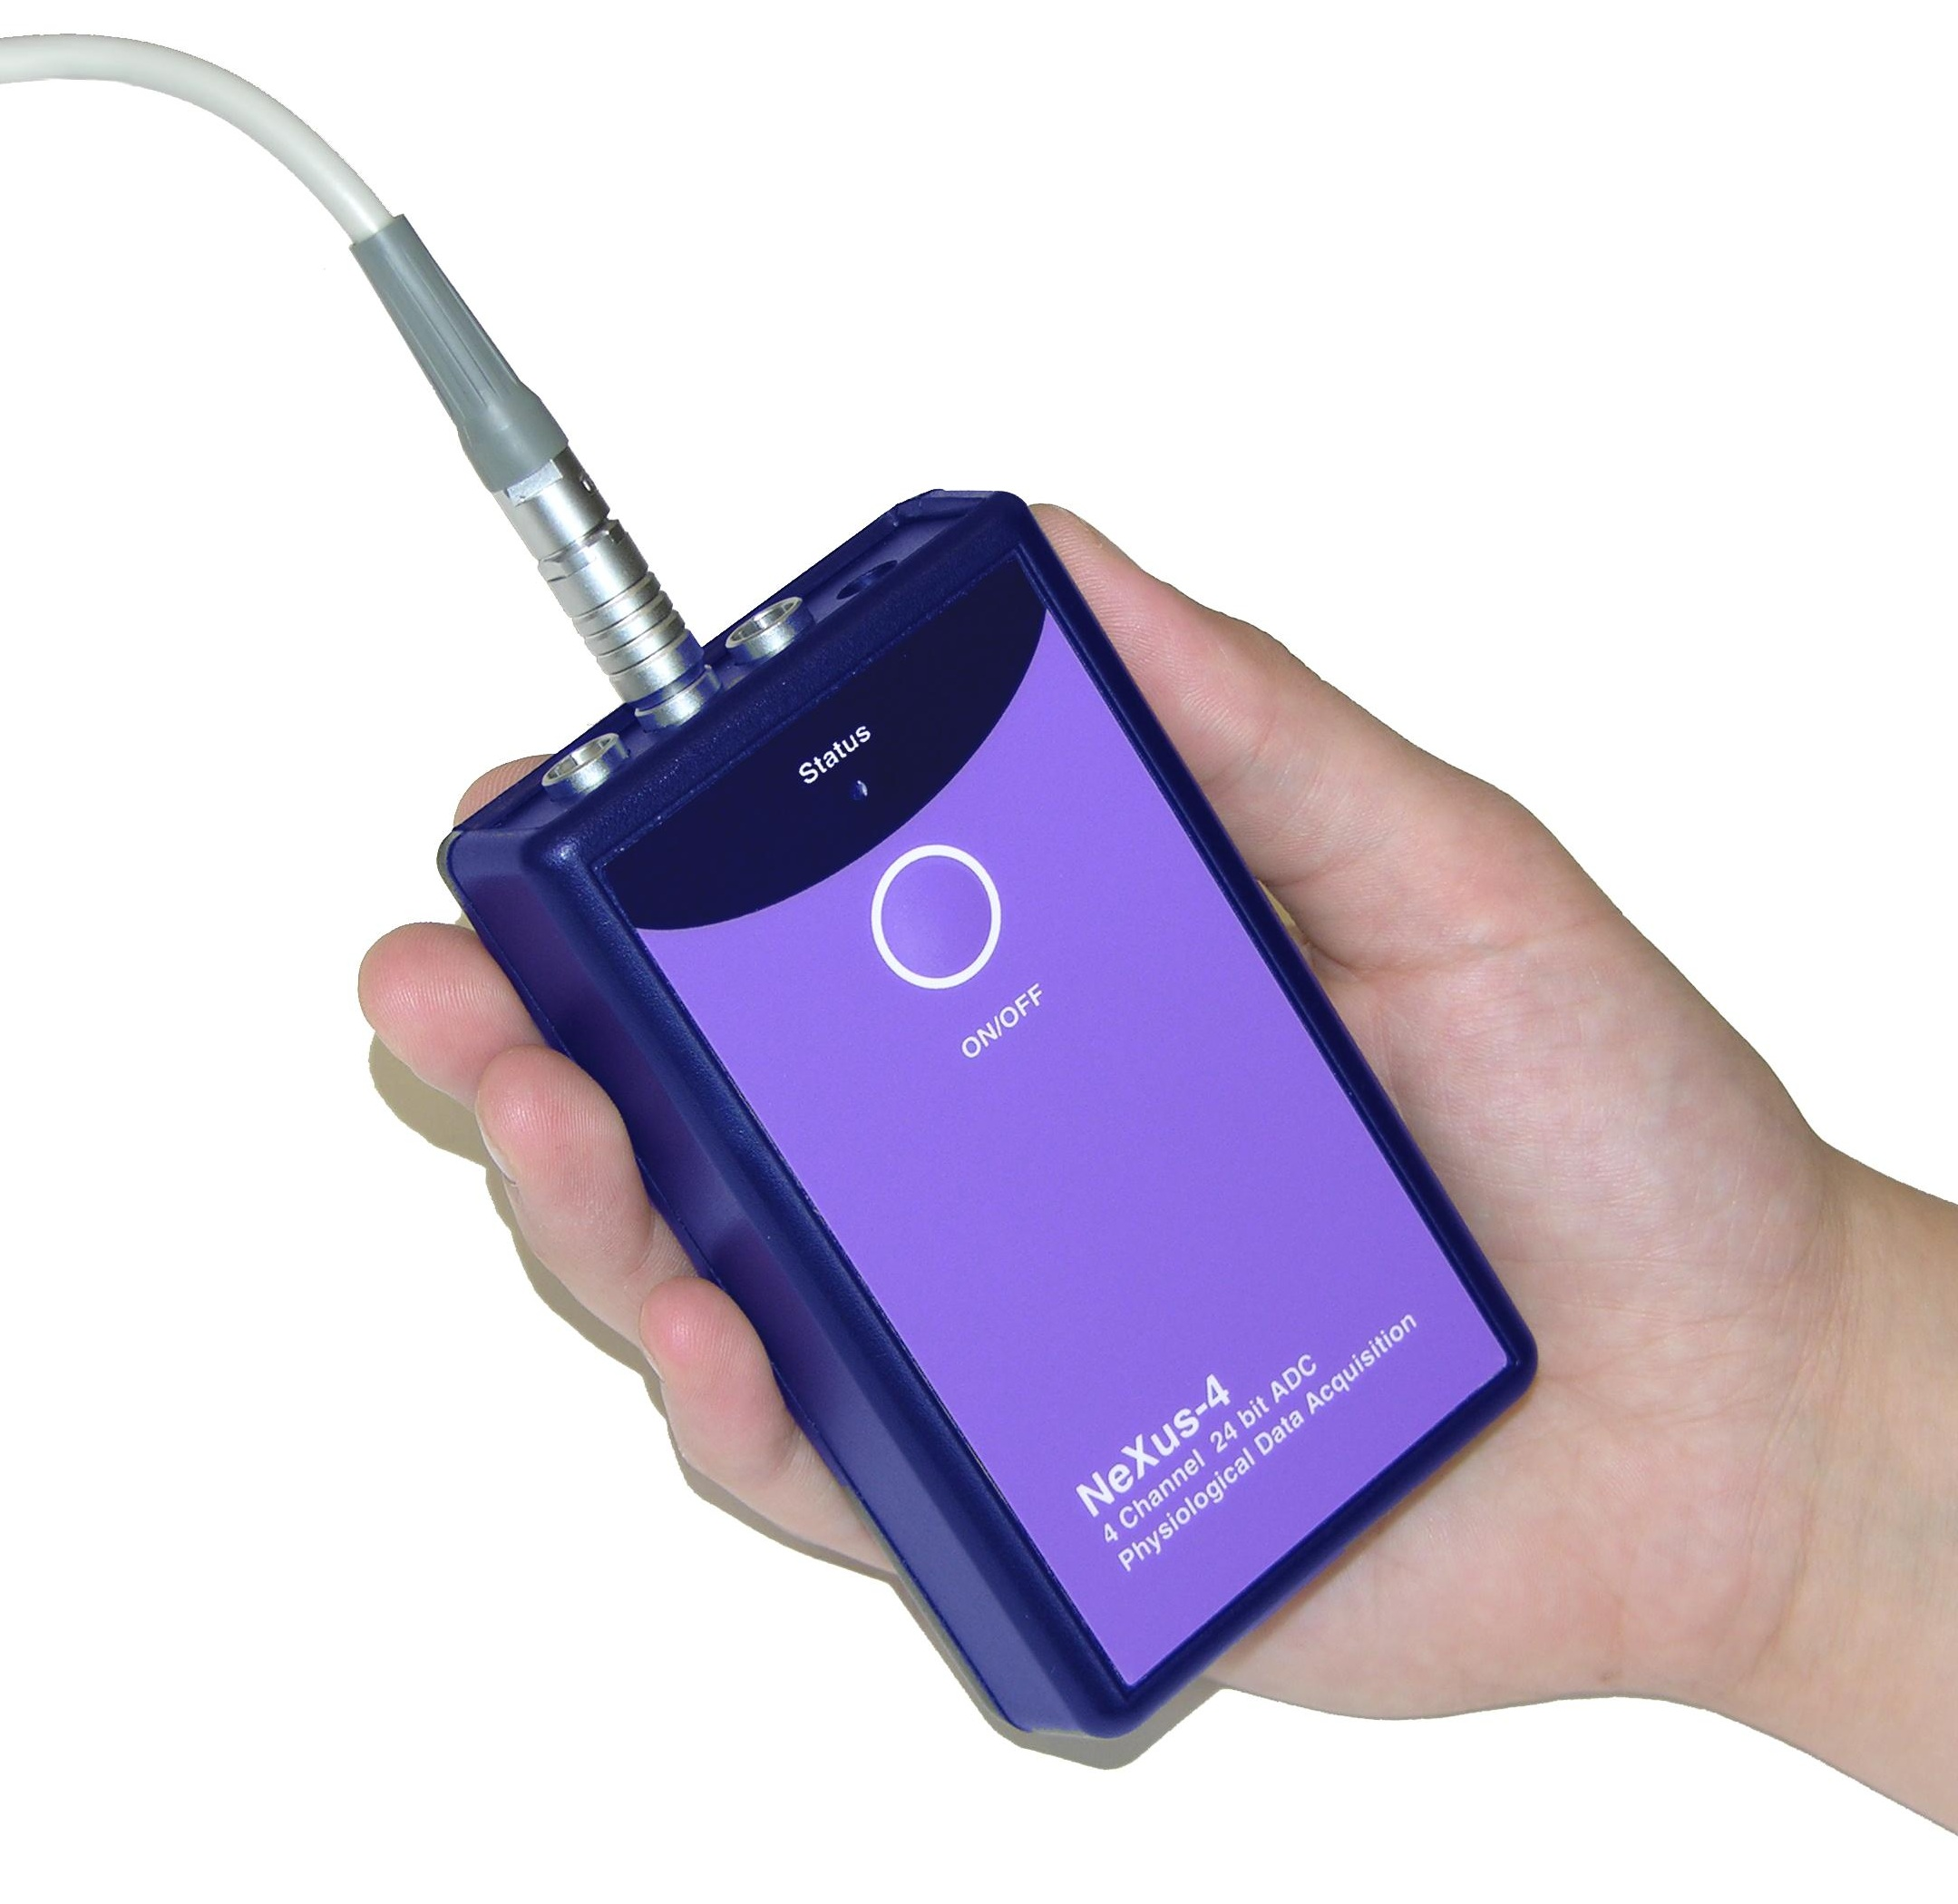
\includegraphics[width=\textwidth] {Figures/nexus.jpg}
		\caption{The Nexus-4 device}
	\end{subfigure}
	
	\vspace{10mm}
	\begin{subfigure}{0.41\textwidth}
		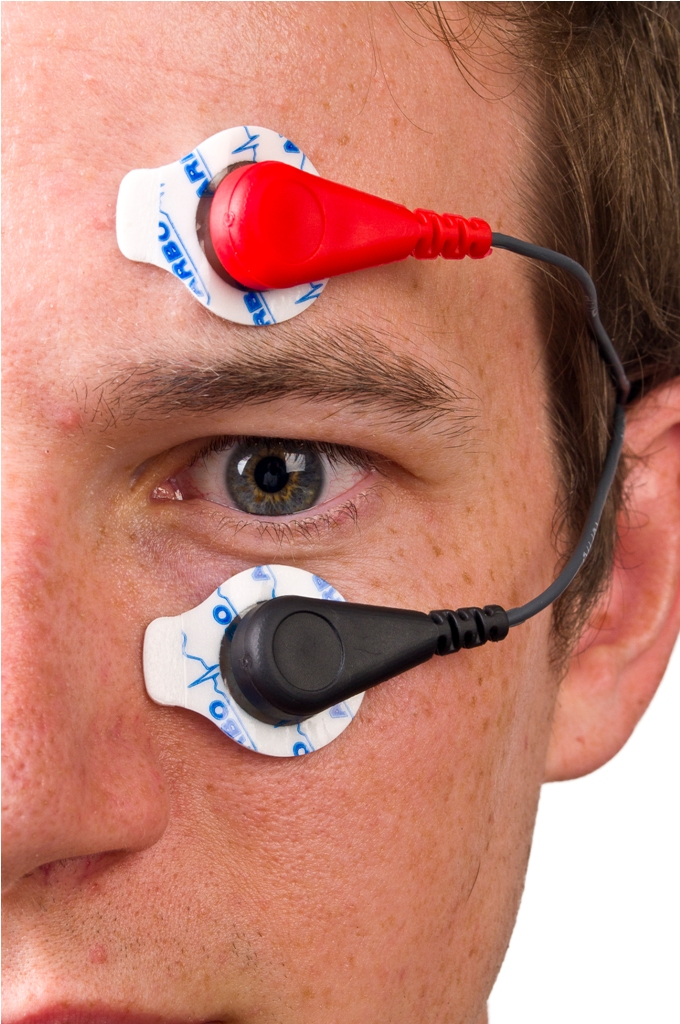
\includegraphics[width=\textwidth] {Figures/nexusEOG.jpg}
		\caption{EOG Sensor}
	\end{subfigure}
	\hfill
	\begin{tabular}{c}
		\begin{subfigure}{0.45\textwidth}
			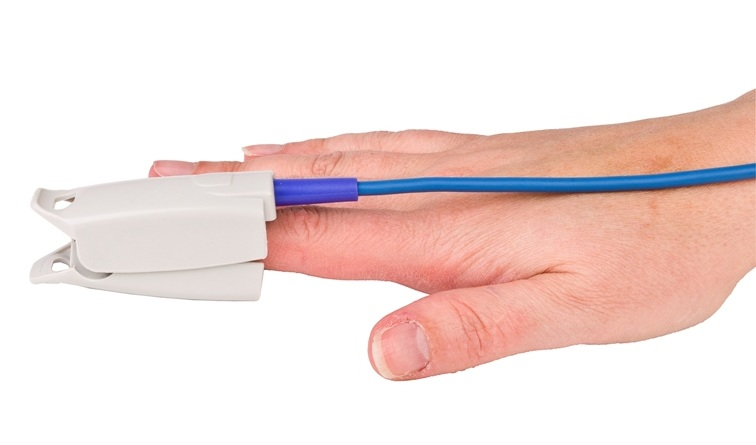
\includegraphics[width=\textwidth] {Figures/nexusBVP.jpg}
			\caption{BVP Sensor}
		\end{subfigure}
		\\
		\begin{subfigure}{0.45\textwidth}
			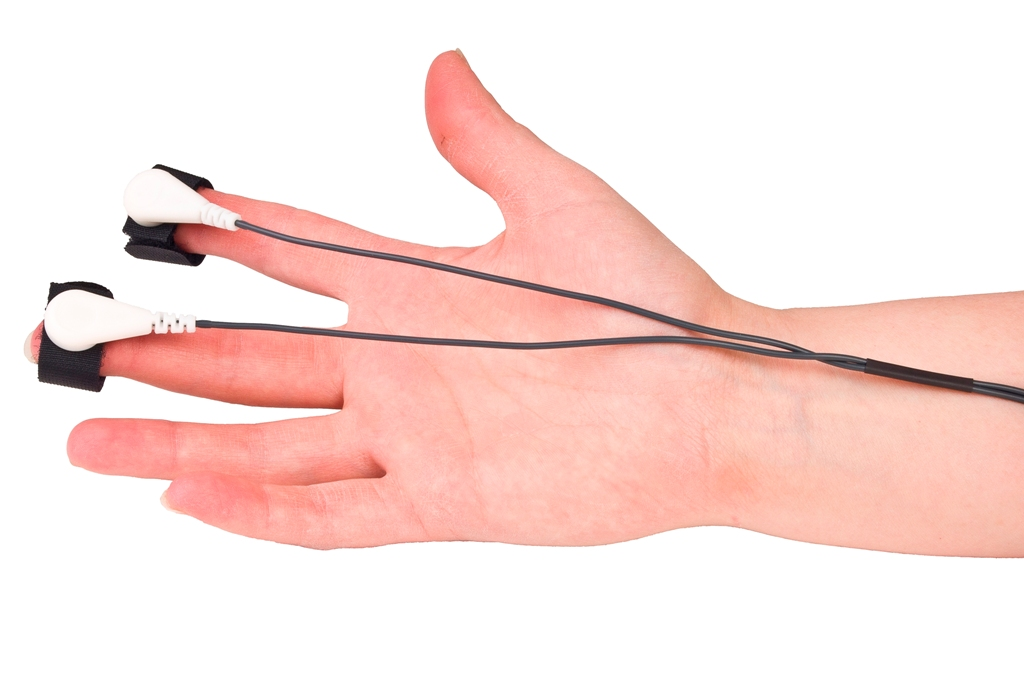
\includegraphics[width=\textwidth] {Figures/nexusSC.jpg}
			\caption{SC Sensor}
		\end{subfigure}
	\end{tabular}
	\caption{The Nexus-4 Wireless Physiological Monitoring System}
	\label{fig:nexus}
\end{figure}

\Cref{fig:laterResponse} is another nice tikz diagram

\begin{figure}[h]
	\centering
	%\tikzset{external/remake next}
	\tikzsetnextfilename{laterResponse}
	\begin{tikzpicture}
		\draw[dashed,black!50!white, name path=thold] (-0.1,0) node[black, anchor=east] {$S_T$}  -- (10,0);
		\draw[blue, name path=rise] (-0.1,-2) node[black,anchor=east] {$S_0$} -- (3,-2) -- (7,1);
		
		\draw[->] (0,-2.2) -- (0,1);
		
		\node[rotate=90, anchor=south] at (-0.8,-1) {\begin{minipage}{4cm}\centering\smaller Posterior probability that \\ stimulus has appeared \end{minipage}};
		
		\draw[->] (3,-3) node[anchor=east] {\smaller Time} -- (4.5,-3);
		
		\path[fill=red, opacity=0.5, name intersections={of=rise and thold}]
			(intersection-1) circle (5pt);
		\draw[<-] (intersection-1) ++(6pt,-6pt) -- ++(0.8,-0.5) node[black, opacity=1,anchor=west] {\smaller Response};
		
		\draw[<-] (3,-2) ++(-0.1,0.1) -- ++(-0.9,0.8) node[anchor=south] {\smaller Stimulus appears};
	\end{tikzpicture}
	\caption{Example LATER response to a stimulus}
	\label{fig:laterResponse}
\end{figure}

\Cref{fig:matlabGsrMetric} is an example of including code. It's not very nice, it was added quite last-minute. But it works.

\begin{figure}[h]
	\centering
	
\begin{minipage}{0.8\textwidth}\smaller\begin{verbatim}
%%%%%%%%%%%%%%%%%%
%% ArousalMetric.m
%%%%%%%%%%%%%%%%%%

% Find peaks and troughs in raw signal
[pks, pLocs] = findpeaks(filtered_signal);
[trs, tLocs] = findpeaks(-filtered_signal);
trs = -trs;

% Trim peaks from the start and troughs from the end of the data
while(pLocs(1) < tLocs(1))
    pLocs(1) = [];
    pks(1) = [];
end

while(tLocs(end) > pLocs(end))
    tLocs(end) = [];
    trs(end) = [];
end

% Calculate arousal metric
peakHeights = pks - trs;
peakWidths = raw_signal_times_secs(pLocs) - raw_signal_times_secs(tLocs);
peakRiseRate = peakHeights ./ peakWidths';
peakValues = peakHeights .* peakRiseRate;

peakEffect = zeros(numel(filtered_signal),1);

peakEffect(pLocs) = peakValues;

arousal_metric = RunningFn(@sum,peakEffect,5000);
\end{verbatim}
	\end{minipage}
	\caption{MATLAB code for computing continuous arousal metric from filtered SC signal.}
	\label{fig:matlabGsrMetric}
\end{figure}

\Cref{fig:gtaSchematic} is another nice tikz diagram.

\pgfdeclarelayer{background}
\pgfdeclarelayer{middle}
\pgfsetlayers{background,middle,main}

\begin{figure}[h]
	\centering
	%\tikzset{external/remake next}	
	\tikzsetnextfilename{gtaSchematic}
	\begin{tikzpicture}

		
		\node (gta) [align=center, blue!50!black,text=black] {Simulation Software\\(GTA)};
		
		\node (script) [below=0.5cm of gta.south, font=\small\sffamily, draw, anchor=north, rounded corners, blue!50!black, fill=blue!5, text=black] {Custom "mission" script};
		
		\begin{pgfonlayer}{middle}
			\node (simulator) [draw, fit={(gta) (script)},inner sep=0.5cm, rounded corners, blue!50!black, fill=blue!2, text=black] {};
		\end{pgfonlayer}
		
		\node (software) [below=2cm of simulator.south, align=center, draw, rounded corners, draw=blue!50!black, text=black, fill=blue!5] {Simulation monitoring \\ and control software};
		
						
		\draw [blue!50!black,line width=1.2pt,decoration={markings, mark=at position 0.4 with {\arrow[scale=1.5]{>}}},postaction=decorate] 
			(script.east) to [out=0, in=0] 
			node [black,auto,pos=0.5,font=\smaller\sffamily,text width=3cm, anchor=south west] {\begin{itemize}\item[$\bullet$] Road position \item[$\bullet$] Heading \item[$\bullet$] Speed \end{itemize}}
			(software.east);
		
		\draw [blue!50!black,line width=1.2pt,decoration={markings, mark=at position 0.4 with {\arrow[scale=1.5]{>}}},postaction=decorate] 
			(software.west) to [out=180, in=180] 
			node [black,auto,pos=0.5,swap,font=\smaller\sffamily,text width=2.5cm,anchor=north east] {\begin{itemize}\item[$\bullet$] Weather \item[$\bullet$] Traffic density \item[$\bullet$] Scenario reset \end{itemize}}
			(script.west);
			
		\coordinate (sideWidth) at (4,0);
		\coordinate (lineLeft) at ($(simulator.south west)!0.5!(software.north west) - (sideWidth)$);
		\coordinate (lineRight) at ($(simulator.south east)!0.5!(software.north east) + (sideWidth)$);
		
		\draw [blue!50!black, line width=2pt, dashed]
			(lineLeft)
			to node[auto,font=\smaller\sffamily] {Network interface} 
			(lineRight);
		
		\begin{pgfonlayer}{background}
			\node [inner sep=0pt,fill=blue!5,fit={(lineLeft) (lineRight) ($(simulator.north) + (0,1)$)}] {};
			\node [inner sep=0pt,fill=blue!10,fit={(lineLeft) (lineRight) ($(software.south) - (0,1)$)}] {};
			\node [inner sep=0pt,line width=10pt,draw=white,rounded corners=10pt,fit={(lineLeft) (lineRight) ($(software.south) - (0,1)$) ($(simulator.north) + (0,1)$)}] {};
		\end{pgfonlayer}
		

	\end{tikzpicture}
	\caption{Driving simulator monitoring and control schematic}
	\label{fig:gtaSchematic}
\end{figure}

You might want to show multiple aligned plots. See \Cref{fig:allGtaEda}.

\begin{figure}
	\centering
	%\tikzset{external/remake next}		
	\tikzsetnextfilename{allGtaEda}
	\begin{tikzpicture}[trim axis group left]
		
		\begin{groupplot}[
			group style={
				group size=3 by 4,
				%vertical sep=1cm,
				xlabels at=edge bottom,
				ylabels at=edge left,
				},
			width=0.35\textwidth,
			height=0.35\textwidth,
			%ymin=40,
			%ymax=100,
			ylabel=Skin conductance,
			ytick=\empty,
			xlabel=Time (seconds),
			axis y line=left,
			axis x line=bottom,
			enlarge x limits=0.05,
			enlarge y limits=0.05,
			title style={anchor=north},
			tick label style={font=\scriptsize\sffamily},
			label style={font=\scriptsize\sffamily},
			title style={font=\scriptsize\sffamily},
			/tikz/line width=0.6pt,
			/tikz/line join=round,
			/tikz/line start=round,
			/tikz/line end=round,
			]
			
			\nextgroupplot[title=Subject 1]
			
			\addplot[blue] file {Data/gtaEDA/S1easyEda.csv};
			\addplot[red] file {Data/gtaEDA/S1hardEda.csv};
			
			\nextgroupplot[title=Subject 2]
			
			\addplot[blue] file {Data/gtaEDA/S2easyEda.csv};
			\addplot[red] file {Data/gtaEDA/S2hardEda.csv};
			
			\nextgroupplot[title=Subject 3]
			
			\addplot[blue] file {Data/gtaEDA/S15easyEda.csv};
			\addplot[red] file {Data/gtaEDA/S15hardEda.csv};
			
			\nextgroupplot[title=Subject 4]
			
			\addplot[blue] file {Data/gtaEDA/S4easyEda.csv};
			\addplot[red] file {Data/gtaEDA/S4hardEda.csv};
			
			\nextgroupplot[title=Subject 5]
			
			\addplot[blue] file {Data/gtaEDA/S5easyEda.csv};
			\addplot[red] file {Data/gtaEDA/S5hardEda.csv};
			
			\nextgroupplot[title=Subject 6]
			
			\addplot[blue] file {Data/gtaEDA/S6easyEda.csv};
			\addplot[red] file {Data/gtaEDA/S6hardEda.csv};
			
			\nextgroupplot[title=Subject 7]
			
			\addplot[blue] file {Data/gtaEDA/S8easyEda.csv};
			\addplot[red] file {Data/gtaEDA/S8hardEda.csv};
			
			\nextgroupplot[title=Subject 8]
			
			\addplot[blue] file {Data/gtaEDA/S9easyEda.csv};
			\addplot[red] file {Data/gtaEDA/S9hardEda.csv};
			
			\nextgroupplot[title=Subject 9]
			
			\addplot[blue] file {Data/gtaEDA/S11easyEda.csv};
			\addplot[red] file {Data/gtaEDA/S11hardEda.csv};
			
			\nextgroupplot[title=Subject 10]
			
			\addplot[blue] file {Data/gtaEDA/S12easyEda.csv};
			\addplot[red] file {Data/gtaEDA/S12hardEda.csv};
			
			\nextgroupplot[title=Subject 11]
			
			\addplot[blue] file {Data/gtaEDA/S13easyEda.csv};
			\addplot[red] file {Data/gtaEDA/S13hardEda.csv};
			
			\nextgroupplot[title=Subject 12]
			
			\addplot[blue] file {Data/gtaEDA/S14easyEda.csv};
			\addplot[red] file {Data/gtaEDA/S14hardEda.csv};
			
							
		\end{groupplot}
		

	\end{tikzpicture}
	\caption[Band-passed skin conductance for all subjects]{Band-passed skin conductance for all subjects in {\color{blue}easy (1)} and {\color{red}hard (6)} conditions. Missing data for subjects 1 and 2 is due to hardware failure.}
	\label{fig:allGtaEda}
\end{figure}


\subsubsection*{A cool diagram}

\Cref{fig:sampleEOG} is a particularly cool use of group plots with lines between coordinate systems...

\begin{figure}
	\centering
	%\tikzset{external/remake next}		
	\tikzsetnextfilename{sampleEOG}
	\begin{tikzpicture}[trim axis left]
		
		\begin{groupplot}[
			group style={
				group size=1 by 3,
				vertical sep=2cm,
				},
			width=0.8\textwidth,
			height=0.5\textwidth,
			ytick=\empty,
			ylabel=Voltage,
			xlabel=Time (seconds),
			axis y line=left,
			axis x line=bottom,
			enlarge x limits=0.05,
			enlarge y limits=0.05,
			]
			
			\nextgroupplot[
				title=Raw EOG,
				title style={anchor=north},
				]
			
			\addplot[blue] file {Data/eogRaw.csv};
			
			\nextgroupplot[
				title=Band-Passed EOG,
				title style={anchor=north},
				]
				
			\addplot[blue] file {Data/eogBandPassed.csv};
			\coordinate (ZoomStartA) at (axis cs:20,\pgfkeysvalueof{/pgfplots/ymin});
			\coordinate (ZoomStartB) at (axis cs:36,\pgfkeysvalueof{/pgfplots/ymin});
			\coordinate (ZoomStartATop) at (axis cs:20,\pgfkeysvalueof{/pgfplots/ymax});
			\coordinate (ZoomStartBTop) at (axis cs:36,\pgfkeysvalueof{/pgfplots/ymax});

			\nextgroupplot[
				xmin=21,
				xmax=35,
				]
			
			\addplot[
				blue,
				line width=1pt, 
				line join=round,
				] file {Data/eogSection.csv};
				
			\coordinate (ZoomEndA) at (axis cs:\pgfkeysvalueof{/pgfplots/xmin},\pgfkeysvalueof{/pgfplots/ymax});
			\coordinate (ZoomEndB) at (axis cs:\pgfkeysvalueof{/pgfplots/xmax},\pgfkeysvalueof{/pgfplots/ymax});				
			\coordinate (ZoomEndABottom) at (axis cs:\pgfkeysvalueof{/pgfplots/xmin},\pgfkeysvalueof{/pgfplots/ymin});
			\coordinate (ZoomEndBBottom) at (axis cs:\pgfkeysvalueof{/pgfplots/xmax},\pgfkeysvalueof{/pgfplots/ymin});				
			
			\addplot[
				only marks, 
				red,
				mark=10-pointed star,
				mark size=6pt,
				] file {Data/eogBlinks.csv};
				
		\end{groupplot}
		
		% Draw zoom box
		\begin{pgfonlayer}{background}
			\path[fill=yellow!20,draw=red!50] 
				(ZoomStartA) -- 
				(ZoomStartATop) -- 
				(ZoomStartBTop) -- 
				(ZoomStartB) .. controls ($(ZoomStartB)+(0,-2)$) and ($(ZoomEndB)+(0,1)$)..
				($(ZoomEndB)-(0,1)$) -- 
				(ZoomEndBBottom) -- 
				(ZoomEndABottom) -- 
				(ZoomEndA) .. controls ($(ZoomEndA)+(0,1)$) and ($(ZoomStartA)+(0,-1)$) ..
				(ZoomStartA);

		\end{pgfonlayer}


	\end{tikzpicture}
	\caption[A typical EOG signal]{A typical EOG signal. The raw signal (top) is bandpassed (middle) and then statically thresholded to find blinks (bottom).}
	\label{fig:sampleEOG}
\end{figure}

\Cref{fig:jazzMuAll} is a nice boxplot which gets all its data from a single file. Use this when each box represents the same number of data points (all the columns in the csv are the same length). \Cref{fig:jazzMuSecondaryTask} draws each box based on a different data file.


\begin{figure}
	\centering
	%\tikzset{external/remake next}		
	\tikzsetnextfilename{jazzMuAll}
	\begin{tikzpicture}[trim axis left]
	

		\appendboxplotvals{Data/jazzMuAll.csv}{0}{1}{Blank}{\myColA}{\boxes}
		\appendboxplotvals{Data/jazzMuAll.csv}{1}{2}{Blank ($n$-back)}{\myColB}{\boxes}
		\appendboxplotvals{Data/jazzMuAll.csv}{2}{3}{Image}{\myColC}{\boxes}
		\appendboxplotvals{Data/jazzMuAll.csv}{3}{4}{Video}{\myColD}{\boxes}
		\appendboxplotvals{Data/jazzMuAll.csv}{4}{5}{Video ($n$-back)}{\myColE}{\boxes}

		\begin{axis}[
			box plot axis,
			width=\textwidth,
			height=0.6\textwidth,
			xtick=data,
			xticklabels from table={\boxes}{name},
			xlabel=Condition,
			ylabel=$\mu\ z$-score,
			ymin=-1.8,
			ymax=1.8,
			];
			\addboxplotboxes{\boxes}
			\addplot[box plot outliers] table \myColA;
			\addplot[box plot outliers] table \myColB;			
			\addplot[box plot outliers] table \myColC;
			\addplot[box plot outliers] table \myColD;			
			\addplot[box plot outliers] table \myColE;			

		\end{axis}
	\end{tikzpicture}

	\caption{Comparison of normalised $\mu$ value for all participants in each $n$-back condition.}
	\label{fig:jazzMuAll}
\end{figure}




\begin{figure}
	\centering
	%\tikzset{external/remake next}		
	\tikzsetnextfilename{jazzMuSecondaryTask}
	\begin{tikzpicture}[trim axis left]
	

		\appendboxplotvals{Data/jazzMuSecondaryTaskSilent.csv}{0}{1}{Silent}{\myColA}{\boxes}
		\appendboxplotvals{Data/jazzMuSecondaryTaskNBack.csv}{0}{2}{$n$-back}{\myColB}{\boxes}

		\begin{axis}[
			box plot axis,
			width=0.6\textwidth,
			height=0.6\textwidth,
			xtick=data,
			xticklabels from table={\boxes}{name},
			xlabel=Condition,
			ylabel=$\mu\ z$-score,
			ymin=-1.8,
			ymax=1.8,
			];
			\addboxplotboxes{\boxes}
			\addplot[box plot outliers] table \myColA;
			\addplot[box plot outliers] table \myColB;			

		\end{axis}
	\end{tikzpicture}

	\caption[Comparison of normalised $\mu$ value for all participants, comparing silent and $n$-back conditions]{Comparison of normalised $\mu$ value for all participants, comparing silent and $n$-back conditions. Silent $\neq\ n$-back ($p<0.001$) }
	\label{fig:jazzMuSecondaryTask}
\end{figure}
	
	





























